\section{MARCO TEORICO} 

\par 


\subsection{Entity Framework}
	\par Entity Framework es un marco de ORM de código abierto para aplicaciones .NET admitidas por Microsoft. Permite a los desarrolladores trabajar con datos utilizando objetos de clases específicas del dominio sin centrarse en las tablas y columnas de la base de datos subyacente donde se almacenan estos datos. Con el Entity Framework, los desarrolladores pueden trabajar en un nivel más alto de abstracción cuando tratan con datos, y pueden crear y mantener aplicaciones orientadas a datos con menos código en comparación con las aplicaciones tradicionales.[2]\\
\\Su arquitectura:
\begin{figure}[H]
\begin{center}
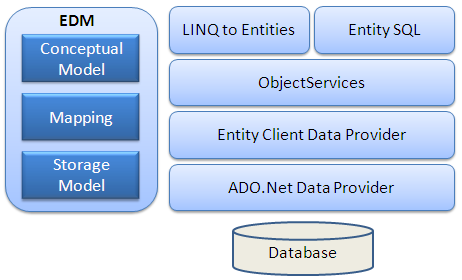
\includegraphics[width=9cm]{./Imagenes/ef-architecture}
\end{center}
\end{figure}

\subsection{API REST}
	\par Ha pasado más de una década desde que Roy Fielding, un científico informático estadounidense y uno de los autores principales de la especificación HTTP, introdujo Representational State Transfer (REST) como un estilo de arquitectura. A lo largo de los años, REST ha ganado impulso gracias a su popularidad para la creación de servicios web.\\
Al no tener estado, y al crear identificadores únicos para permitir el almacenamiento en caché, la creación de capas y la capacidad de lectura, las API REST hacen uso de los verbos HTTP existentes (GET, POST, PUT y DELETE) para crear, actualizar y eliminar nuevos recursos. El término REST se usa con frecuencia para describir cualquier URL que devuelva JSON en lugar de HTML.

\subsection{ Consultas LINQ}
	\par Permite consultar cualquier objeto  enumerable en ADO.NET mediante el uso del modelo de programación de Language-Integrated Query (LINQ) [1] para recuperar datos de la base de datos subyacente. El proveedor de la base de datos traducirá estas consultas LINQ al lenguaje de consulta específico de la base de datos (por ejemplo, SQL para una base de datos relacional).\\
Hay 3 tecnologias ADO.NET LINQ distintas:
\begin{itemize}
	\item LINQ to DataSet: proporciona una capacidad de consulta mas rica y optimizada sobre DataSet.
	\item LINQ to SQL: permite consultar directamente los esquemas de las base de datos de SQL Server.
	\item LINQ to Entities: permite consultar Entity Data Model.
\end{itemize}

\subsection{Pruebas Unitarias}
	\par Las pruebas unitarias son la mejor forma de probaar el codigo de una aplicación a lo largo de su desarrollo. Estas pruebas permiten asegurar que losmétodos devuelven resultados correctos, teniendo en cuenta los argumentos que se le pasan y, además, se pueden utilizar para hacer Test Driven Development. Se trata de una técnica en la que se escriben antes que las clases y los métodos.[4]\\
 No obstante, tras realizar la integración con otros módulos deberá revisarse de nuevo la interfaz.